\documentclass[10pt]{article}

\usepackage[a4paper,top=4cm,bottom=2.7cm,left=2.5cm,right=2.5cm]{geometry}
\usepackage{amsmath,amssymb}
\usepackage{booktabs}
\usepackage{graphicx}
\usepackage{url}
\usepackage[hidelinks]{hyperref}
\setlength{\emergencystretch}{2em}

\title{A Coefficient-Aware Finite-Difference Benchmark for Solver Selection and CPU/GPU Stencil Scaling in Heat-Conduction Simulation}

\author{Dong Liu*\\
University of Nottingham Ningbo China\\
Ningbo, China\\
\texttt{ssydl3@nottingham.edu.cn}}

\date{}

\begin{document}
\maketitle

\begin{abstract}
Sparse solves for variable-coefficient heat conduction depend on coefficient geometry, forcing, preconditioner setup, and implementation. We present a verified finite-difference benchmark with an invariant-preserving audit of solver-choice claims. Smooth manufactured solutions recover second-order convergence and an aligned interface test verifies flux treatment. Beyond a baseline coefficient-family comparison, matched binary fields hold contrast, material fraction, total variation, and maximum log-gradient fixed. In a controlled N = 192, contrast-1000 case, translating the same two-island field by one grid point raises Jacobi-PCG iterations from 403 to 677 and reverses the setup-inclusive winner from Jacobi to AMG in all five repeats. Reflection-invariant Krylov subspaces explain why an odd source can avoid slow island modes; source perturbations and an independent motif family test this interpretation. An interleaved audit with classical AMG confirms that reversal locations depend on the candidate solver set. All 2956 controlled extension solves satisfy an independently checked relative residual below 1e-8. The resulting audit exposes limits of translation-invariant coefficient descriptors without proposing a new solver-selection algorithm. A separate paired callback calibration quantifies monitoring overhead without treating historical and controlled timings as interchangeable. CPU/CUDA measurements separately quantify stencil scaling; GPU claims remain restricted to resident-data kernels. Raw CSV files, scripts, tests, and generated outputs support the numerical and performance claims.
\end{abstract}

\section{Introduction}

Discretising heat conduction with spatially varying conductivity produces sparse linear systems whose solution cost depends on the coefficient field, mesh resolution, forcing and preconditioning. Repeated stencil evaluations introduce a separate implementation cost. A useful benchmark must verify the discretisation and specify which parts of these computations are timed.

We test whether coefficient summaries and grid resolution distinguish the measured solver choices. Matched coefficient fields, translations and source perturbations provide controlled tests of their limitations.

The benchmark solves the steady heat-conduction equation with spatially varying conductivity. Manufactured solutions verify the smooth cases; inclusion, layered and checkerboard fields test the solvers with discontinuous conductivity. The implementation uses Python, NumPy, SciPy, PyAMG, Numba, and Numba-CUDA for sparse solves and CPU/GPU stencil implementations \cite{Virtanen2020,Harris2020,Lam2015,Bell2023}.

Prior numerical-analysis texts establish the convergence properties of finite-difference discretisations and the role of Krylov and multigrid methods in sparse PDE solves \cite{Strikwerda2004,Hestenes1952,Saad2003,Briggs2000,Ruge1987}. Recent sparse and PDE solver studies further underline that preconditioning, sparse matrix execution, and accelerator mapping remain active constraints for modern workloads \cite{Bernaschi2026EnergySparseMultiGPU,Welter2026HDGGPUPreconditioning}; recent AMG and diffusion-solver work targets communication cost and coefficient difficulty more directly \cite{Yuan2025CRAMG,Green2022AnisotropicDiffusionSolver}. General reproducible-benchmarking work provides principles for automated reruns and evidence retention \cite{Koskela2023ReproBenchmark}. Here, numerical verification, coefficient descriptors and archived timings connect solver choices to the tested PDE and implementation. Combining PDE verification with performance benchmarking is established practice.

The contribution is a controlled audit within an existing finite-difference benchmark. Numerical verification and baseline solver/stencil measurements establish the implementation. An exact matched-field construction then tests whether standard coefficient descriptors distinguish solver difficulty. Translation controls preserve shape and topology as well as scalar descriptors, while forcing and transpose controls separate source symmetry from matrix and implementation effects. The resulting counterexamples are connected to preconditioned spectra and setup-inclusive costs. The study introduces no new PDE, discretisation, Krylov method, AMG algorithm, or GPU kernel; coefficient-aware denotes an auditable interpretation of measured cases, not an online selection algorithm.

\section{Related Work}

The closest benchmark precedents already combine elliptic problems and solver performance. HPGMG-FV solves variable-coefficient elliptic problems on Cartesian grids and supports CPU and accelerator execution \cite{SPECHPGMG2021}. AMG2023 benchmarks finite-difference diffusion with BoomerAMG and Krylov methods; its performance denominator includes setup time plus a specified number of solves \cite{LLNLAMG2023}. Setup-inclusive timing is therefore an established practice. The present study addresses a narrower question through a small coefficient-family grid, explicit interface checks, and a complete record of measured solver choices. These systems provide methodological context; no performance comparison against HPGMG or hypre is claimed.

Finite-difference methods provide a direct route from elliptic and parabolic PDEs to sparse linear systems on structured grids \cite{Strikwerda2004}. For self-adjoint diffusion operators, conservative flux forms are especially useful because face-based coefficient averaging preserves the symmetry and locality expected by Krylov methods. Once discretised, the main computational problem is sparse linear algebra rather than pointwise equation evaluation.

The conjugate-gradient method remains a baseline solver for symmetric positive definite systems \cite{Hestenes1952,Saad2003}. Its performance depends strongly on spectral conditioning, which generally deteriorates under mesh refinement and can be strongly affected by coefficient contrast and geometry. Multigrid methods reduce this sensitivity by addressing error components across scales \cite{Briggs2000}. Algebraic multigrid extends that idea to matrix-defined problems without requiring a hand-built geometric hierarchy \cite{Ruge1987}. In this study, PyAMG is used as an accessible Python implementation of algebraic multigrid \cite{Bell2023}.

Performance portability is a separate concern. NumPy provides high-level array operations, SciPy provides sparse linear algebra, and Numba compiles numerical Python kernels to machine code \cite{Harris2020,Virtanen2020,Lam2015}. CUDA exposes massively parallel GPU execution, but launch overhead and data movement can erase speedups on small problems \cite{NvidiaCudaGuide2026,NumbaCudaDocs2026}. Recent stencil and CUDA kernel studies report sensitivity to memory traffic, kernel structure, and problem size \cite{Pekkila2025StencilGPUs,Makhmut2026CUDABuckleyLeverett}. The benchmark therefore reports GPU results as resident-data kernel measurements for repeated updates where data stay on the device, and it keeps raw evidence for independent reruns \cite{Koskela2023ReproBenchmark}.

High-contrast preconditioning and isolated-island modes already have analytical foundations \cite{Aksoylu2008,AksoyluYeter2009}. Krylov convergence depends on the spectral distribution and its excitation by the initial residual, so a condition number alone can be misleading \cite{Carson2024}. Recent material-aware smoothed aggregation explicitly targets heterogeneous interfaces \cite{Firmbach2026}. More generally, algorithm-selection studies recognise performance variation among instances with identical features \cite{Ewald2011}. Our extension applies these established ideas to an exact matched-field and translation audit, quantifying their consequences for verified heat-conduction solves and setup-inclusive choices. Neither source dependence nor feature insufficiency is claimed as a new general theorem.

\section{Mathematical Model and Discretisation}

The model problem is the steady heat-conduction equation
\begin{equation}
    -\nabla\cdot(k(x,y)\nabla u(x,y)) = f(x,y), \quad (x,y)\in (0,1)^2,
    \label{eq:pde}
\end{equation}
with homogeneous Dirichlet boundary conditions unless otherwise stated. The coefficient $k(x,y)$ represents spatially varying thermal conductivity. The smooth test uses
\begin{equation}
    k(x,y)=1+0.5\sin(2\pi x)\sin(2\pi y),
\end{equation}
and the high-contrast stress test uses a circular inclusion,
\begin{equation}
    k(x,y)=1+99\,\mathbf{1}_{(x-0.5)^2+(y-0.5)^2<0.15^2}.
\end{equation}
For the decision-map study, this pair is expanded into a parameterised coefficient grid. The smooth family uses $k=1+a\sin(2\pi x)\sin(2\pi y)$ with $a=(C_k-1)/(C_k+1)$, giving target contrast $C_k$. The inclusion, layered, and checkerboard families use piecewise values in $\{1,C_k\}$ with $C_k\in\{10,30,100\}$, while the smooth family uses $C_k\in\{3,10,30\}$ and the constant case gives $C_k=1$. The layered field changes at $y=1/2$; the checkerboard uses eight blocks per coordinate direction. The circle has radius 0.15 and centre $(1/2,1/2)$.

To report contrast, coefficient sharpness, and coefficient geometry separately, each coefficient field is summarised by
\begin{equation}
    C_k=\frac{\max k}{\min k},\qquad
    G_k^{(h)}=\|\nabla_h\log k\|_{\infty},\qquad
    V_k=\frac{\sum |\Delta_x k|+\sum |\Delta_y k|}{N-1},
    \label{eq:difficulty}
\end{equation}
Here $G_k^{(h)}$ is the maximum nodal Euclidean magnitude of the log-gradient, using centred interior differences and first-order one-sided boundary differences. Here $\Delta_x k$ and $\Delta_y k$ are unscaled nearest-neighbour differences over all nodal pairs in each coordinate direction; $V_k$ divides their absolute sums by $N-1$ and is used only as a grid-normalised total-variation proxy. For discontinuous coefficient fields, $G_k^{(h)}$ depends on the grid spacing and is interpreted at fixed $N$ rather than as a continuous invariant. Small-grid spectral evidence is also recorded through computed condition-number estimates $\kappa(A)=\lambda_{\max}(A)/\lambda_{\min}(A)$.

The domain is discretised on an $N\times N$ uniform grid with spacing $h=1/(N-1)$. Interior unknowns are ordered lexicographically. For an interior node $(i,j)$, the conservative five-point stencil is
\begin{align}
(Au)_{i,j} ={}&
k_{i+1/2,j}\frac{u_{i,j}-u_{i+1,j}}{h^2}
+k_{i-1/2,j}\frac{u_{i,j}-u_{i-1,j}}{h^2} \nonumber\\
&+k_{i,j+1/2}\frac{u_{i,j}-u_{i,j+1}}{h^2}
+k_{i,j-1/2}\frac{u_{i,j}-u_{i,j-1}}{h^2},
\label{eq:stencil}
\end{align}
where face coefficients use arithmetic averages of adjacent nodal values in the main two-dimensional decision map. Arithmetic averaging defines the primary two-dimensional benchmark operator; harmonic averaging probes sensitivity to the interface treatment. For discontinuous coefficient fields, harmonic face averaging is also implemented and tested as a sensitivity check, because it matches the series-resistance interpretation of one-dimensional layered conduction. The shared positive face weights give a sum of weighted squared nodal differences in the discrete energy. With boundary values fixed, both choices produce sparse symmetric positive definite systems for positive $k$ and homogeneous Dirichlet boundaries.

Arithmetic faces are retained to preserve the specified nodal graph-diffusion benchmark and its historical comparisons, not because they are the preferred interface law for composite heat conduction. Interface conductivity is a standard numerical heat-transfer issue \cite{Patankar1980}. For two half-links of equal length with conductivities a and b, continuity of flux gives the series resistance h/(2a) + h/(2b), hence $k_H = 2ab/(a+b)$, whereas $k_A=(a+b)/2$. Their difference is $(a-b)^2/[2(a+b)]$: it is $O(h^2)$ for smooth positive conductivity, but need not be small at a jump. At contrast c = 100, $k_A/k_H=(c+1)^2/(4c)=25.5025$ on a mixed link. This is a local conductance ratio under the half-link interface assumption, not a global temperature-error estimate. Thus the arithmetic high-contrast results describe solver behaviour for that discrete operator; they do not validate composite-material heat flux. Harmonic averaging has the correct aligned series-resistance interpretation, while a curved interface requires additional geometric treatment. The matched-field audit includes both averages so that its conclusions are not restricted to arithmetic faces.

For smooth convergence verification, the exact solution is
\begin{equation}
    u_{\mathrm{exact}}(x,y)=\sin(\pi x)\sin(\pi y),
\end{equation}
and $f$ is generated analytically for the constant and smooth coefficient cases. Errors are reported as the interior-node root-mean-square (normalised discrete $L^2$) and maximum norms. The observed convergence rate is obtained by a least-squares fit of $\log(e)$ against $\log(h)$. A separate one-dimensional verification problem uses $k(x)=k_1$ for $x<1/2$ and $k(x)=k_2$ for $x>1/2$ with $u(0)=0$ and $u(1)=1$. Its analytic solution is piecewise linear and satisfies continuity of both $u$ and $k u_x$ at the interface; this test isolates whether arithmetic and harmonic face averages respect the expected interface flux.

\section{Solver and Implementation Methods}

The assembled sparse matrix is solved with three methods: unpreconditioned CG, Jacobi-preconditioned CG, and algebraic-multigrid preconditioned CG. The AMG case uses the tested PyAMG default smoothed-aggregation hierarchy as a V-cycle preconditioner for SciPy CG; this should be read as one concrete AMG configuration rather than a claim about all AMG parameter choices. The recorded PyAMG 5.3.0 defaults use symmetric strength, standard aggregation, Jacobi prolongation smoothing with omega = 4/3, symmetric block Gauss-Seidel pre/post smoothing, at most ten levels, and a coarse-grid limit of ten unknowns. Historical runs did not fix the random starts used in PyAMG spectral-radius estimation, so exact hierarchy-dependent results can vary across reruns. Manufactured-solution runs use a relative residual tolerance of $10^{-11}$ so that solver error does not dominate discretisation error; solver-comparison runs use SciPy CG with relative tolerance $10^{-8}$, zero absolute tolerance, the default zero initial guess, and a maximum of 12000 iterations in the decision map. The baseline coefficient-family solver comparisons use the same deterministic unit right-hand side at a given grid size, so the right-hand side is controlled across cases. The controlled extension below separately varies the right-hand side, which can excite different spectral components. The reported time separates preconditioner setup from iterative solve time and also gives the total time. Matrix assembly and right-hand-side construction are excluded from these times. Iterative solve times include a callback that recomputes the true relative residual after every iteration, adding one sparse matrix-vector product and norm evaluations per iteration. The reported selections and speedups therefore apply to this monitored implementation. Methods are run in a fixed order, and the first AMG setup in a fresh process also includes the PyAMG import; these timings do not isolate hierarchy construction from first-use overhead. BLAS thread settings and processor power states were not recorded, limiting exact performance replication. Failed convergence would be recorded as a structured row in the raw CSV artefact, although all baseline benchmark cases converged.

Three evidence groups have distinct timing meanings \cite{Hoefler2015}. Historical coefficient-family results include a true-residual evaluation at every iteration, fixed method order and the first PyAMG import inside setup; their thread settings were not recorded. The controlled matched-field extension uses warm imports, shuffled order, one BLAS thread, paired setup seeds and count-only callbacks, with rtol = 1e-9 and independently checked residual at most 1e-8. The new callback calibration holds the arithmetic operator, unit source, three candidate methods, rtol = 1e-8, warm imports, one BLAS thread and setup seeds fixed, changing only the callback within each pair. All three groups exclude matrix assembly and source construction, and include fresh preconditioner setup in total time. Historical speedups are monitored-implementation results; translation reversals and empirical cost floors are within-extension comparisons. Neither time ratios nor winner boundaries are pooled across these groups. The calibration estimates callback sensitivity under its stated conditions; it cannot retrospectively separate historical import, ordering, threading or machine-state effects.

Matrix-free performance is measured with a separate stencil apply matching Eq.~\eqref{eq:stencil}. Three CPU paths are compared: NumPy vectorisation, Numba serial compilation, and Numba parallel compilation with controlled thread counts. Throughput is reported as an estimated stencil bandwidth using a fixed byte model: 11 double-precision values per interior point for the variable-coefficient stencil, or 88 bytes per point. The Jacobi crossover uses five double-precision values per interior point, or 40 bytes per point. These estimates are operational metrics for comparing implementations of the same stencil family, not hardware peak-bandwidth or direct DRAM-transaction claims.

The CUDA experiment uses a repeated Jacobi update rather than the full variable-coefficient operator. This isolates a simple memory-bound stencil and avoids conflating kernel throughput with sparse-solver algorithmics. CPU and GPU arrays are allocated once, one batch is used for warm-up, and timing continues for at least three batches and 0.2 s. CUDA uses 16 by 16 thread blocks and the Numba CPU baseline uses four threads. These are within-run averages, not independent timing replicates. CUDA timings use a host wall-clock timer around resident-data batches of 20 updates, including Python launch overhead and device synchronisation after each batch. Allocation, compilation warm-up, and host-device transfers are excluded. This boundary matches repeated time-stepping or smoother-like updates where data remain resident on the device, but it should not be read as end-to-end application speedup.

For a single solve, the decision map compares setup-plus-solve times. For coefficient case $c$, grid size $N$, and method set $\mathcal{S}$, it selects
\begin{equation}
    s^*(c,N)=\arg\min_{s\in\mathcal{S}}\left[T_{\mathrm{setup}}(s,c,N)+T_{\mathrm{solve}}(s,c,N)\right],
    \label{eq:decision}
\end{equation}
among converged runs. This is a retrospective measured comparison: all candidates have already been run, and the winning time excludes the cost of evaluating the other candidates. This makes one-time AMG setup cost visible rather than treating iteration count as the only outcome. It is not a repeated-right-hand-side reuse model; such a model would require an explicit solve count $m$.

We report Spearman rank correlations between $C_k$, $G_k^{(h)}$, $V_k$, the available-grid condition estimate, CG iterations, and the speedup of the selected solver over CG. The coefficient set is a designed benchmark grid rather than a random sample from a defined population, so rank correlations are treated as descriptive association diagnostics rather than population-level inferential estimates. Pooled rows summarise all case-size entries but are not treated as independent samples because the same coefficient family appears at multiple grid sizes. Fixed-$N$ rows provide the safer coefficient-level reading and include deterministic case-resampling intervals. Iteration-count associations are treated as the primary solver-difficulty diagnostic; associations with selected-solver speedup are secondary and exploratory because the full decision grid uses a single timing pass per cell. Permutation $p$-values are archived in the CSV as diagnostics rather than used to claim pairwise descriptor separation. Timing stability is assessed by repeating selected decision-map cases five times and then reporting the solver chosen by median total time, the per-repeat vote fraction, and the relative interquartile range of the selected method. The full decision grid remains a single-pass benchmark, while the repeat check probes whether the most important decisions are robust or near ties. The hardware crossover model is similarly bounded: for the repeated Jacobi kernel it fits $T(n)=\alpha+\beta n$, where $n=(N-2)^2$, and archives the global four-point fit as an exploratory summary rather than a validated local crossover model.

\section{Experiments and Results}

All experiments were run on Windows 11 with Python 3.12.9, NumPy 2.4.6, SciPy 1.18.1, Numba 0.67.0, PyAMG 5.3.0, and Numba-CUDA 0.30.4. The machine used an AMD Ryzen 9 7940HS w/ Radeon 780M Graphics CPU with 8 physical cores and 16 logical processors, approximately 16 GB of system memory reported by the operating system as 15.2 GB usable, and an NVIDIA GeForce RTX 4060 Laptop GPU with compute capability 8.9. The exact raw CSV outputs, environment metadata, and scripts are included in the supplementary artefact. The decision map covers 13 coefficient cases, three grid sizes, and three Krylov/preconditioner choices. The spectral conditioning study uses $N=32,64,128$. Extremal eigenvalues of the unpreconditioned matrix are estimated with SciPy eigsh (smallest/largest algebraic eigenvalue, tolerance 1e-6, maximum 20000 iterations). These estimates do not describe the preconditioned operator; the N = 256 correlations using an N = 128 spectral proxy are cross-resolution diagnostics. The rank-correlation analysis uses all 39 case-size decisions and three fixed-grid strata of 13 cases; condition numbers are matched to $N=64$ and $N=128$ where available, and the $N=128$ condition estimate is used as the maximum-available case-level spectral proxy for $N=256$. The repeated timing check uses five repeats for one constant case and four nonconstant representative cases at each of the three decision-grid sizes, covering 15 case-size cells. The face-averaging sensitivity study reruns the three discontinuous $C_k=100$ stress cases with arithmetic and harmonic face averages at $N=64,128,256$.

\subsection{Verification and Coefficient Difficulty}

The manufactured-solution study confirms the expected second-order behaviour of the finite-difference scheme. Table~\ref{tab:convergence} reports fitted rates using $N=32,64,128,256$ with a CG residual tolerance of $10^{-11}$. Both the constant and smooth variable-coefficient cases produced $L^2$ rates close to two. Figure~\ref{fig:convergence} gives the same result as a log-log error plot.

\begin{table}[t]
\centering
\caption{Manufactured-solution convergence for the finite-difference discretisation.}
\label{tab:convergence}
\resizebox{\columnwidth}{!}{%
\begin{tabular}{lrrrr}
\toprule
Case & $p_{L^2}$ & $p_{\infty}$ & Finest $L^2$ & Residual \\
\midrule
Constant coefficient & 2.01 & 2.00 & $6.35\times10^{-6}$ & $1.60\times10^{-12}$ \\
Smooth variable coefficient & 2.02 & 2.00 & $6.39\times10^{-6}$ & $2.01\times10^{-11}$ \\
\bottomrule
\end{tabular}
}
\end{table}


\begin{figure}[t]
\centering
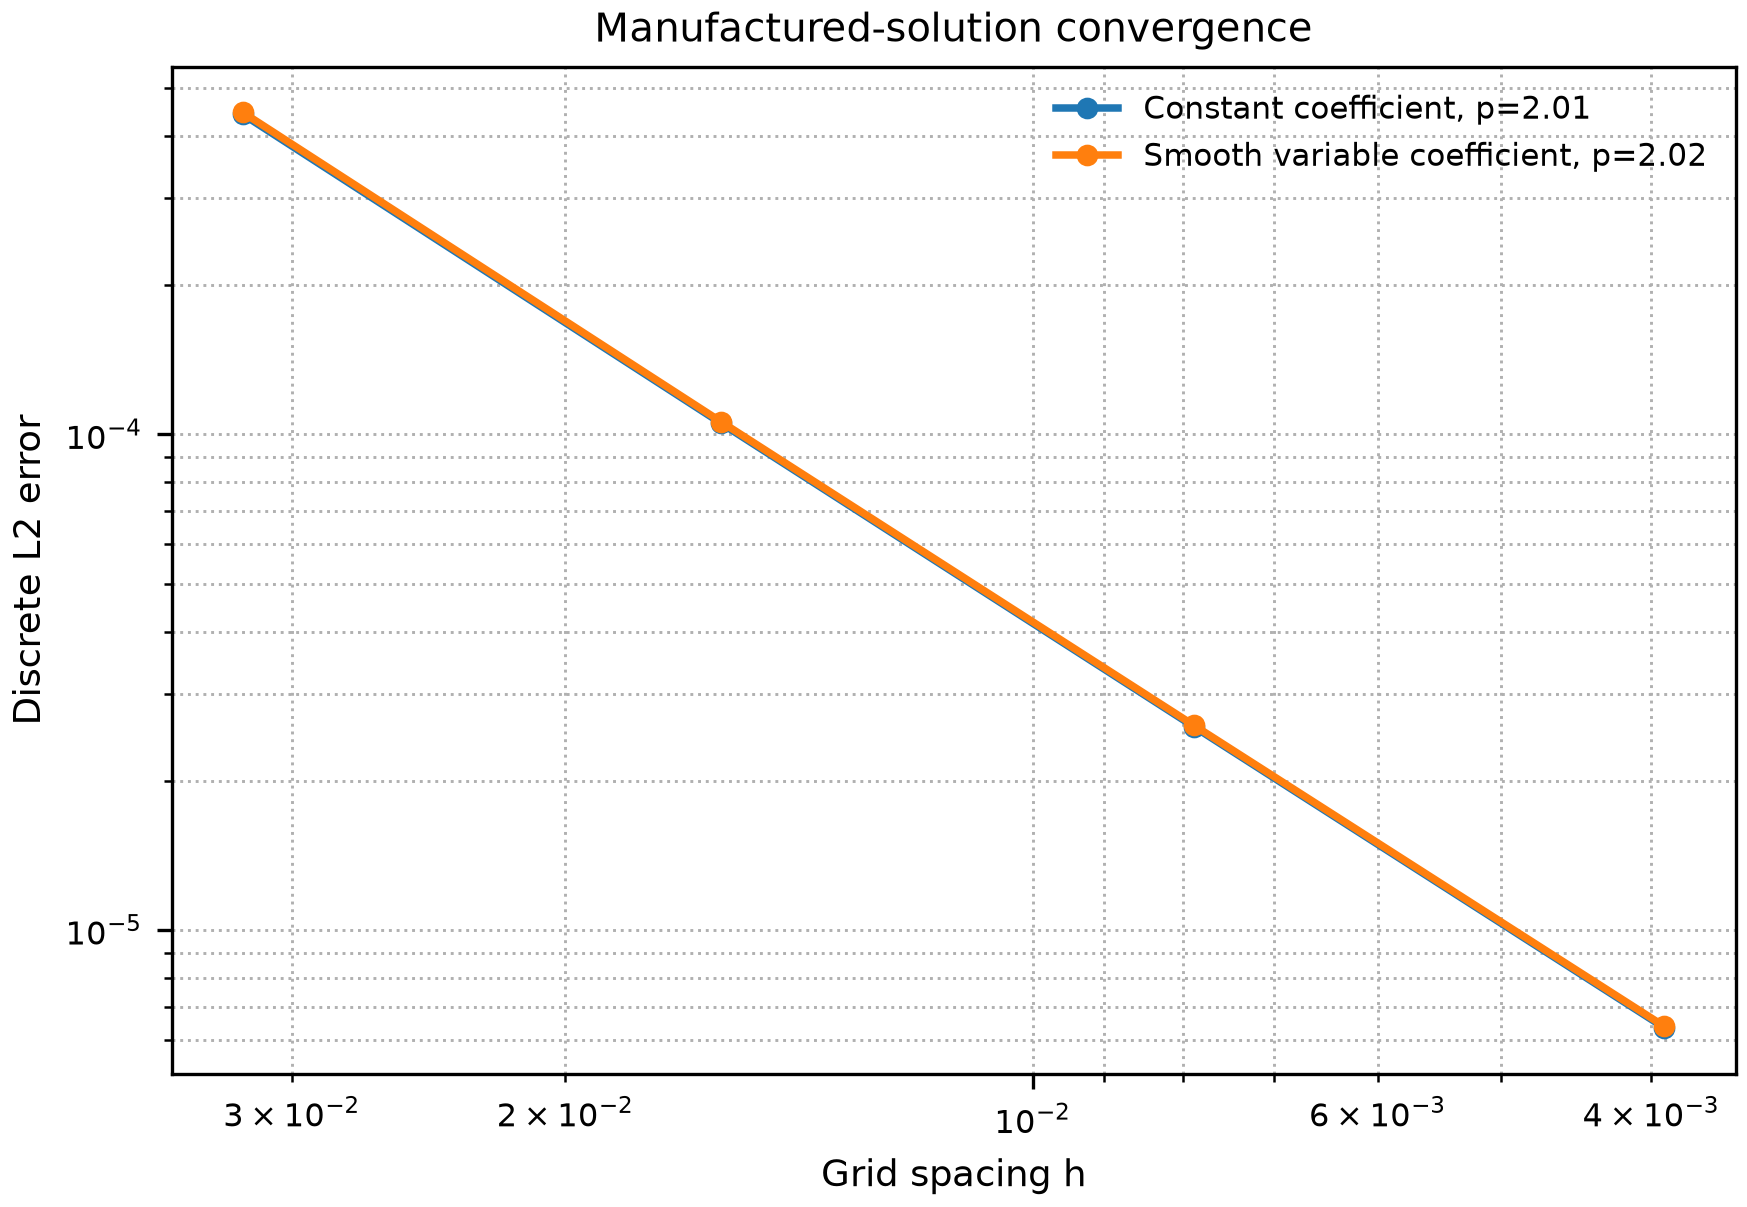
\includegraphics[width=0.84\linewidth]{figures/convergence_l2.png}
\caption{Manufactured-solution convergence of the finite-difference operator.}
\label{fig:convergence}
\end{figure}

The discontinuous-interface check in Table~\ref{tab:interface-verification} isolates a different error mechanism. For an aligned one-dimensional two-material conduction problem, harmonic face averaging reproduced the analytic interface flux to roundoff, while arithmetic averaging showed a grid-refined interface error. This does not make harmonic averaging a universal choice for all multidimensional discontinuities, but it prevents the benchmark from relying only on smooth manufactured-solution evidence.

\begin{table}[t]
\centering
\caption{Discontinuous-interface verification on a one-dimensional two-material heat-conduction problem. Harmonic face averaging recovers the analytic flux continuity to roundoff in this aligned-interface test.}
\label{tab:interface-verification}
\resizebox{\columnwidth}{!}{%
\begin{tabular}{rrrrr}
\toprule
$N$ & $L^2$ error, arithmetic & $L^2$ error, harmonic & Flux error, arithmetic & Flux error, harmonic \\
\midrule
32 & $1.27\times10^{-2}$ & $5.96\times10^{-16}$ & $6.33\times10^{-2}$ & $5.11\times10^{-15}$ \\
64 & $6.21\times10^{-3}$ & $1.56\times10^{-15}$ & $3.07\times10^{-2}$ & $6.66\times10^{-15}$ \\
128 & $3.07\times10^{-3}$ & $3.55\times10^{-14}$ & $1.51\times10^{-2}$ & $2.44\times10^{-14}$ \\
256 & $1.53\times10^{-3}$ & $9.51\times10^{-15}$ & $7.49\times10^{-3}$ & $4.91\times10^{-14}$ \\
\bottomrule
\end{tabular}
}
\end{table}


Table~\ref{tab:difficulty} reports representative coefficient descriptors. The spectral evidence confirms that contrast alone is not a complete difficulty measure. At $N=128$, the inclusion case with $C_k=100$ had a computed condition-number estimate of $6.43\times10^5$, while the checkerboard case with the same contrast had a much smaller estimate of $3.12\times10^4$ under this discretisation. Figure~\ref{fig:conditioning} shows the same effect across the measured coefficient grid.

\begin{table}[t]
\centering
\caption{Representative coefficient-difficulty descriptors. Metrics use $N=64$ for the discrete descriptors; $\kappa(A)$ is the largest available spectral estimate, here $N=128$.}
\label{tab:difficulty}
\resizebox{\columnwidth}{!}{%
\begin{tabular}{llrrrr}
\toprule
Case & Family & $C_k$ & $G_k^{(h)}$ & TV proxy & $\kappa(A)$ \\
\midrule
constant & Constant & 1.0 & 0.00 & 0.00 & $6.54\times10^{3}$ \\
smooth\_c30 & Smooth & 29.7 & 16.41 & 4.76 & $1.38\times10^{4}$ \\
inclusion\_c100 & Inclusion & 100.0 & 205.15 & 113.14 & $6.43\times10^{5}$ \\
layered\_c100 & Layered & 100.0 & 145.06 & 100.57 & $2.61\times10^{5}$ \\
checkerboard\_c100 & Checkerboard & 100.0 & 205.15 & 1408.00 & $3.12\times10^{4}$ \\
\bottomrule
\end{tabular}
}
\end{table}


\begin{figure}[t]
\centering
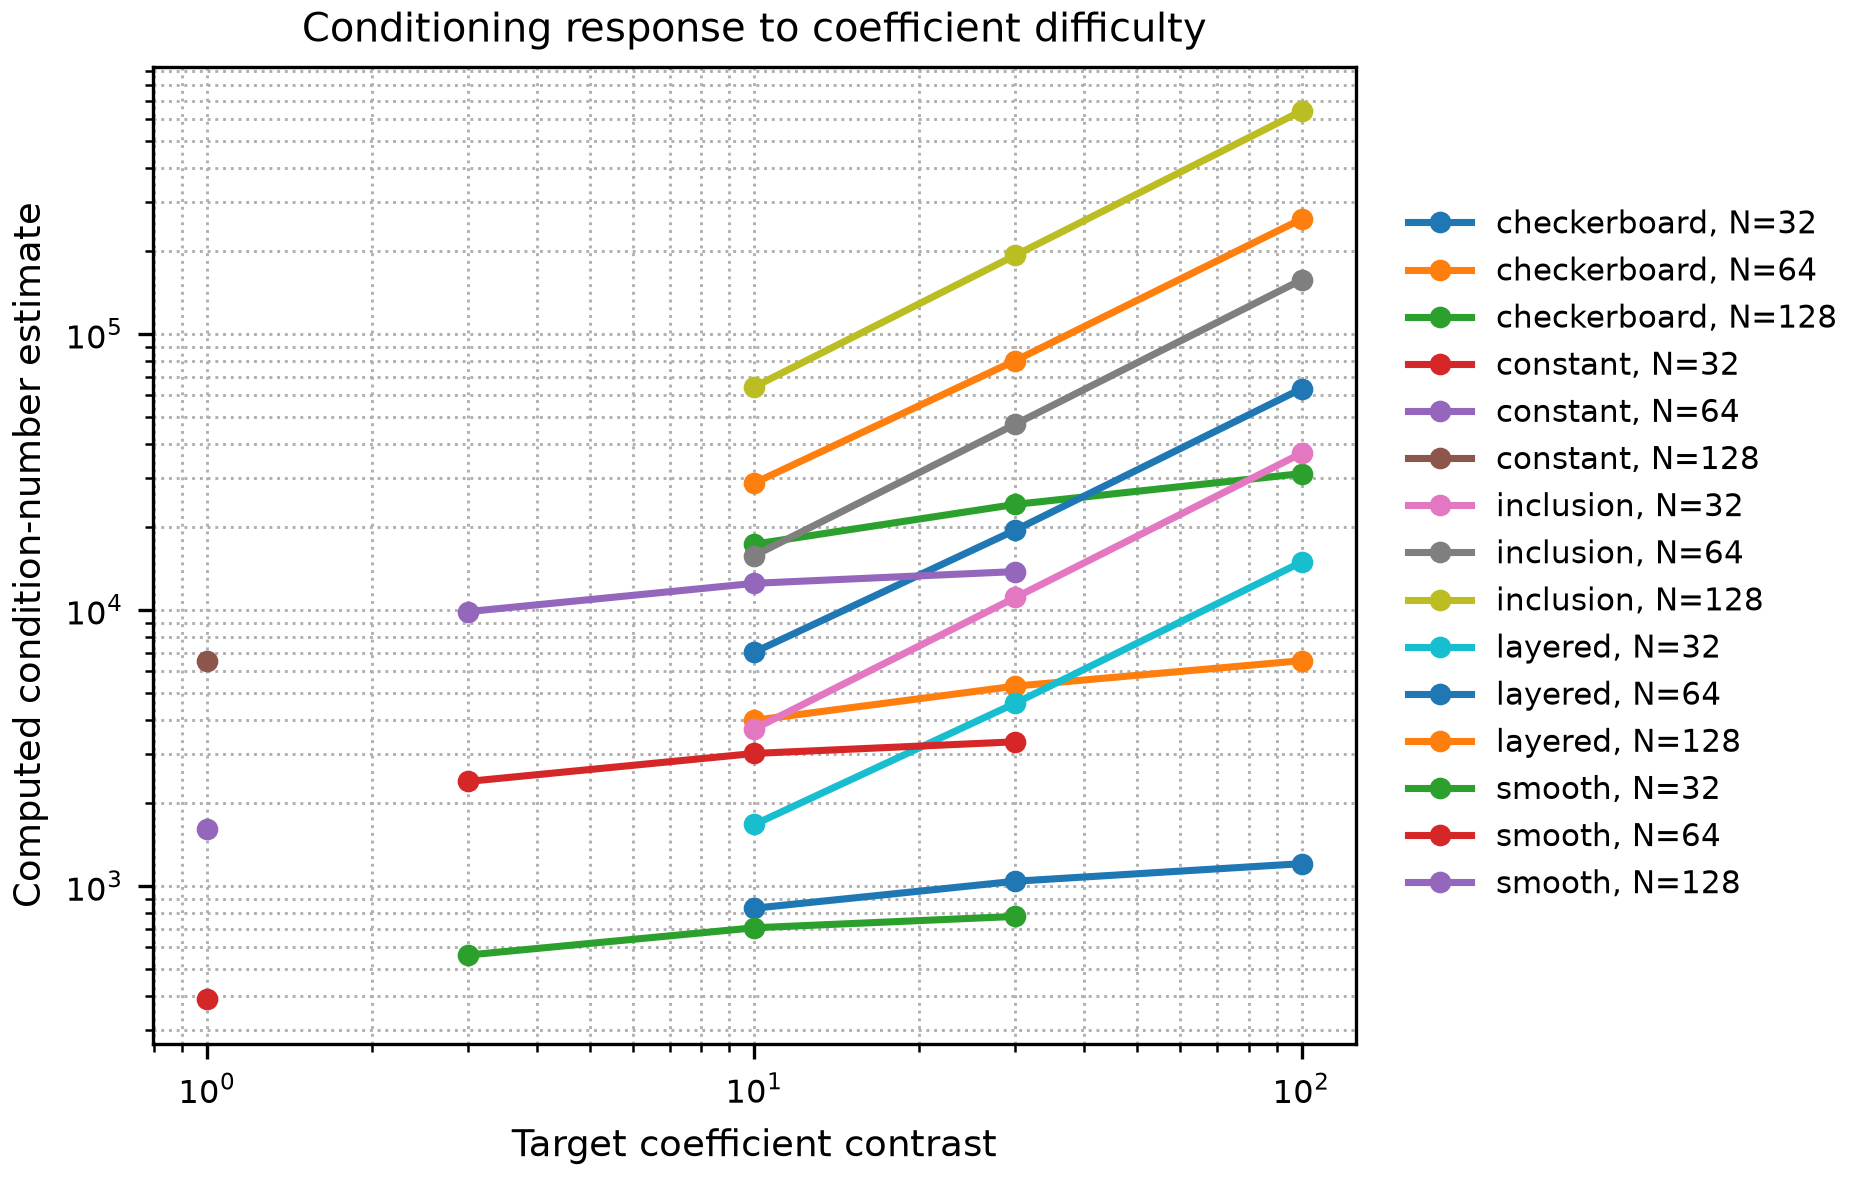
\includegraphics[width=0.84\linewidth]{figures/conditioning.png}
\caption{Computed condition-number response to coefficient contrast and coefficient geometry.}
\label{fig:conditioning}
\end{figure}

The supplementary rank-correlation table distinguishes pooled size effects from fixed-grid coefficient comparisons. The matched condition estimate has pooled correlation 0.94 with selected-solver speedup, but fixed-grid samples contain only 13 cases and their case-resampling intervals overlap. These are descriptive ordering signals, not population confidence guarantees. The matched-field audit below tests descriptor sufficiency directly, rather than inferring it from pooled correlation.


\subsection{Solver Decision Map and Preconditioner Effect}

The single-pass setup-inclusive decision map records a resolution-dependent outcome. Within each grid size the winning class is the same across all tested coefficient fields, so this map supplies no evidence that descriptors improve prediction of the winner beyond resolution alone. Over the 13 coefficient cases, Jacobi-PCG was fastest in every $N=64$ run, while AMG-PCG was fastest in every $N=128$ and $N=256$ run. Table~\ref{tab:decision-summary} summarises this transition. The median speedup of the selected solver over CG increased from $2.79\times$ at $N=64$ to $7.80\times$ at $N=256$, and the largest speedup reached $25.72\times$ for the layered $C_k=100$ case. Because each decision-map cell uses one timing pass, this map is interpreted together with the repeated representative cases below.

\begin{table}[t]
\centering
\caption{Setup-inclusive single-solve decision summary over the coefficient-family grid. Counts report the fastest converged method by setup-plus-solve time from one timing pass per cell.}
\label{tab:decision-summary}
\resizebox{\columnwidth}{!}{%
\begin{tabular}{rrrrrrr}
\toprule
$N$ & Cases & CG & Jacobi-PCG & AMG-PCG & Median speedup vs CG & Max speedup vs CG \\
\midrule
64 & 13 & 0 & 13 & 0 & 2.79 & 6.76 \\
128 & 13 & 0 & 0 & 13 & 5.44 & 19.40 \\
256 & 13 & 0 & 0 & 13 & 7.80 & 25.72 \\
\bottomrule
\end{tabular}
}
\end{table}



The complete arithmetic/harmonic sensitivity results are reported below in Table~
ef{tab:face-main}.



The supplementary timing-stability table reports all 15 case-size cells in the existing repeated-timing dataset. The median-best solver also won all five individual repeats in 14 cells: Jacobi-PCG for the four nonconstant N = 64 cases, and AMG-PCG for all five cases at both N = 128 and N = 256. The constant N = 64 cell is a near tie: the median favours Jacobi-PCG by only $1.03\times$, while CG wins four repeats. For constant conductivity on this uniform grid, the diagonal is a scalar multiple of the identity; Jacobi therefore does not improve the spectral condition number and yields equivalent CG iterates in exact arithmetic. The archived single-pass CG and Jacobi-PCG iteration counts agree at all three sizes. Their small-grid timing difference is not evidence of an iteration-reduction benefit.



Solver behaviour changed substantially when the coefficient field became high contrast. At $N=256$, unpreconditioned CG required 4370 iterations in the high-contrast case, compared with 770 iterations in the smooth case. Jacobi preconditioning reduced the high-contrast iteration count to 535, while AMG-PCG reduced it to 12. Total time fell from 6.155 s for CG to 0.288 s for AMG-PCG in the high-contrast case. Table~\ref{tab:solver} summarises the finest-grid comparison, and Fig.~\ref{fig:solver_runtime} shows total-time scaling across grid sizes. The iteration-scaling figure is retained in the supplementary artefact.

\begin{table}[t]
\centering
\caption{Solver comparison at $N=256$ grid points in each direction.}
\label{tab:solver}
\resizebox{\columnwidth}{!}{%
\begin{tabular}{llrrr}
\toprule
Case & Method & Iter. & Time (s) & Rel. residual \\
\midrule
Smooth variable & CG & 770 & 0.939 & $9.71\times10^{-9}$ \\
Smooth variable & Jacobi-PCG & 605 & 0.829 & $9.88\times10^{-9}$ \\
Smooth variable & AMG-PCG & 9 & 0.240 & $4.82\times10^{-9}$ \\
High contrast & CG & 4370 & 6.155 & $9.95\times10^{-9}$ \\
High contrast & Jacobi-PCG & 535 & 0.728 & $9.14\times10^{-9}$ \\
High contrast & AMG-PCG & 12 & 0.288 & $4.44\times10^{-9}$ \\
\bottomrule
\end{tabular}
}
\end{table}


\begin{figure}[t]
\centering
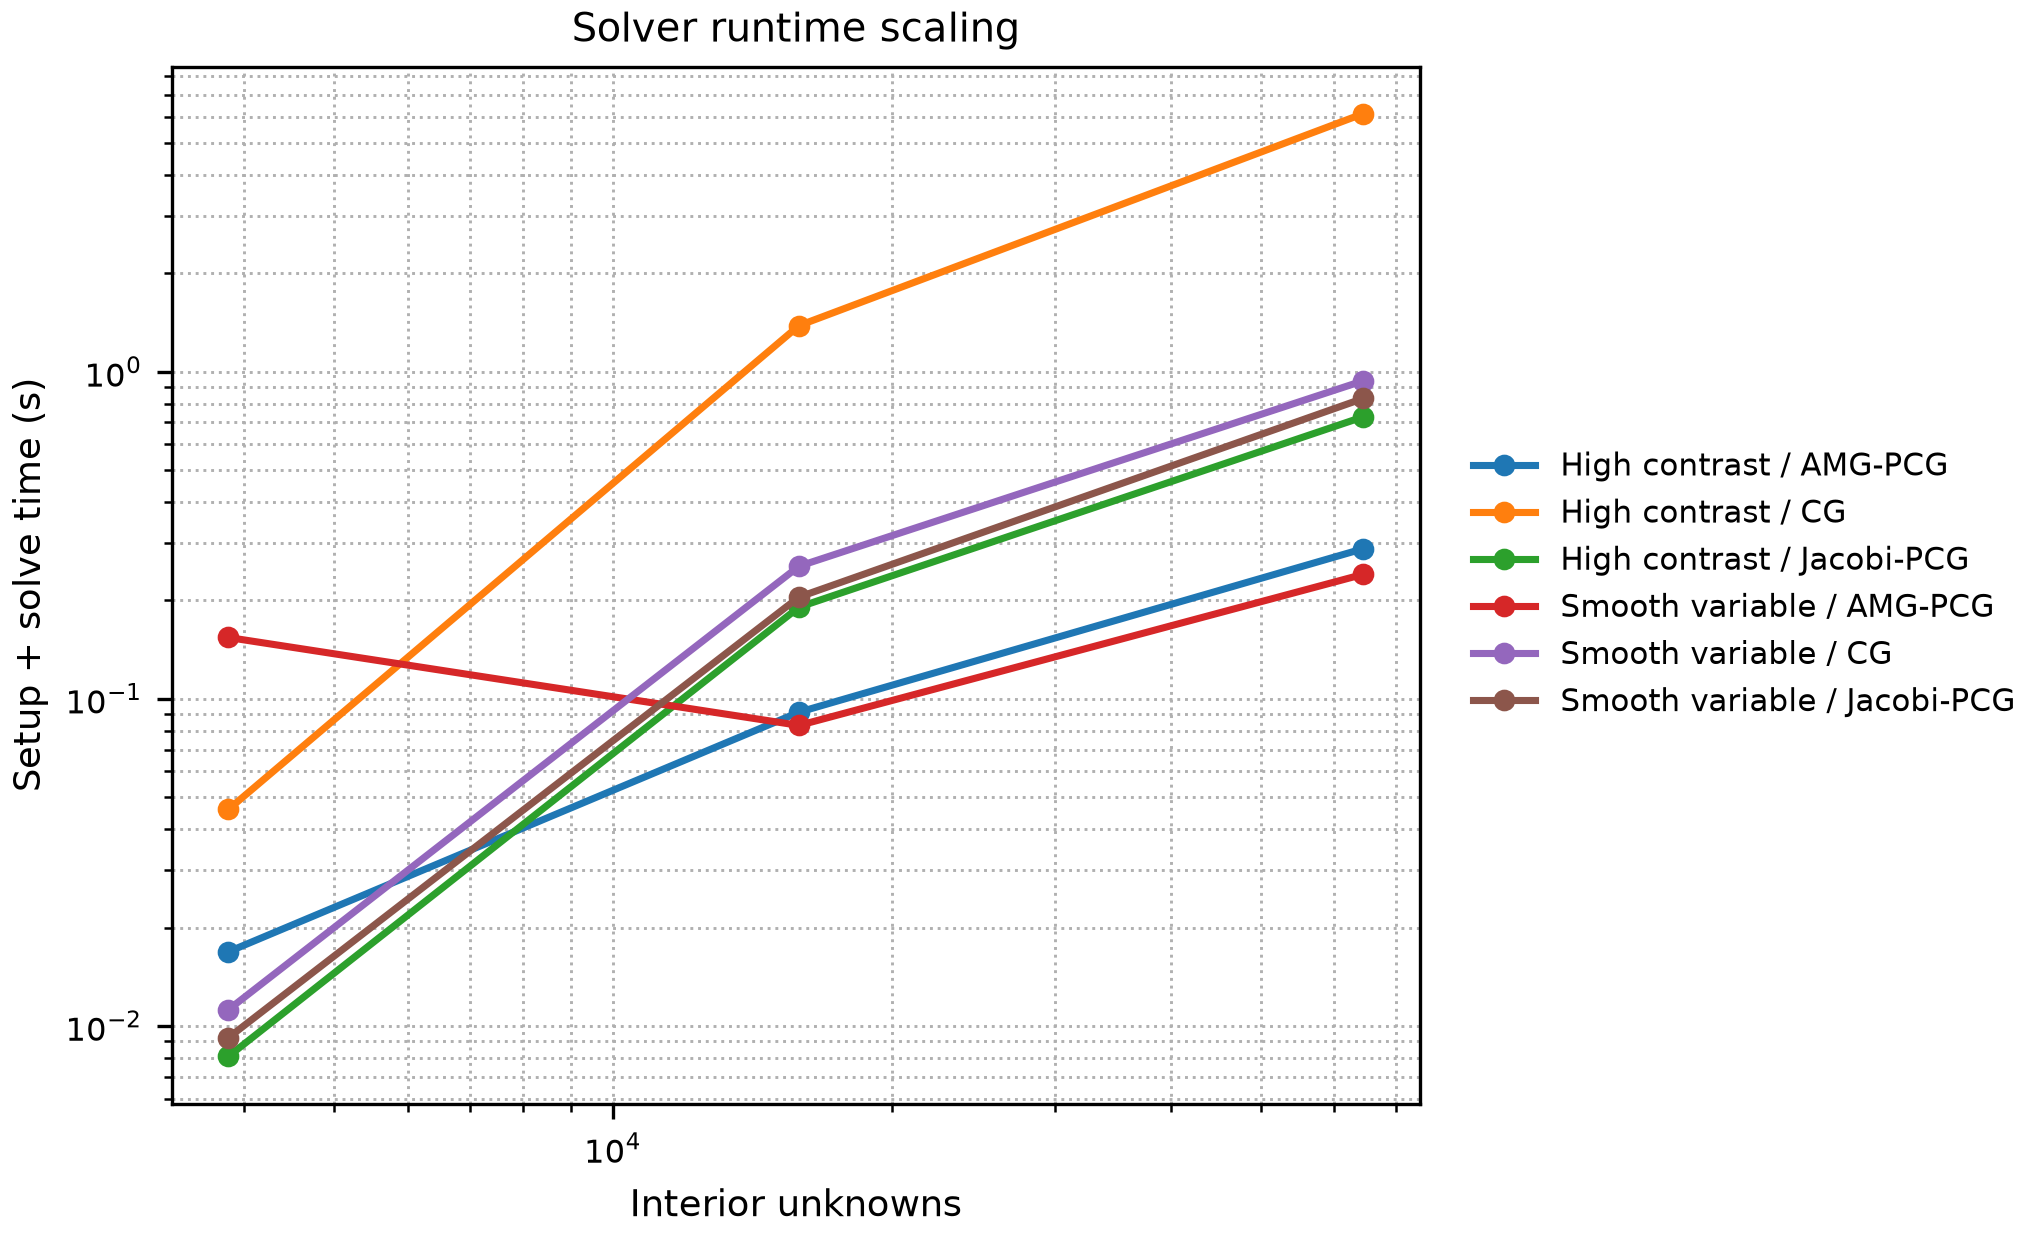
\includegraphics[width=0.84\linewidth]{figures/solver_runtime.png}
\caption{Total setup plus solve time for CG, Jacobi-PCG, and AMG-PCG.}
\label{fig:solver_runtime}
\end{figure}


The complete face-averaging check in Table \ref{tab:face-main} reports all nine historical case-size cells. Arithmetic/harmonic iteration counts differ substantially, including AMG changes for checkerboard fields, although the setup-inclusive winner is unchanged in these single passes. Agreement of winners does not establish physical equivalence of the operators, timing stability, or identical solution accuracy. The aligned one-dimensional verification and the two-dimensional solver-cost sensitivity answer separate questions.

\input{tables/face_sensitivity_main}

\subsection{Paired Callback Calibration}

A prospective calibration covers constant, inclusion and checkerboard conductivity (contrast 100 for the latter two), N = 64, 128, 256, three methods, two callback modes and seven repeats: 378 recorded solves. Each repeat shuffles all 54 jobs; each solve constructs a fresh preconditioner with a seed matched across callback modes. Every run satisfies the independent residual threshold of 1e-8. All 189 paired solutions have identical byte hashes and iteration counts. Median paired monitored/count-only solve-time ratios range from 1.54 to 1.84 for CG, 1.58 to 1.77 for Jacobi-PCG, and 1.03 to 1.06 for AMG-PCG. These method-dependent penalties change reported speedups even when the median winner is unchanged.

Table \ref{tab:protocol} reports every case-size cell, including vote instability. The median winner agrees between callbacks in all nine cells. At constant N = 256, however, count-only AMG wins only three of seven repeats despite having the lowest method median; the median winner and majority vote answer different questions. The archived method summaries retain setup, solve and total-time quartiles for all candidates. Several N = 128 winners differ from the historical map under both callback modes, so callback removal alone cannot explain the historical-to-calibration difference. No universal N = 128 AMG crossover is inferred. The calibration does not measure cold-import overhead or control operating-system, power or thermal variation.

\begin{table}[htbp]
\centering
\caption{Paired callback calibration. Winner entries give method, median total milliseconds and votes out of seven. Last columns give median paired monitored/count-only solve-time ratios. J = Jacobi-PCG; SA = AMG-PCG.}
\label{tab:protocol}
\small
\begin{tabular}{lllllll}
\toprule
Case & $N$ & Monitored & Count-only & CG & J & SA \\
\midrule
Constant & 64 & CG 5.64 (7/7) & CG 3.55 (5/7) & 1.58 & 1.58 & 1.05 \\
Constant & 128 & CG 31.22 (6/7) & CG 19.11 (7/7) & 1.67 & 1.70 & 1.04 \\
Constant & 256 & SA 141.18 (7/7) & SA 147.70 (3/7) & 1.84 & 1.76 & 1.04 \\
Inclusion & 64 & J 6.67 (7/7) & J 4.12 (7/7) & 1.63 & 1.62 & 1.03 \\
Inclusion & 128 & J 38.28 (7/7) & J 22.34 (7/7) & 1.72 & 1.61 & 1.04 \\
Inclusion & 256 & SA 156.23 (7/7) & SA 152.34 (6/7) & 1.79 & 1.77 & 1.03 \\
Checkerboard & 64 & J 8.69 (6/7) & J 5.63 (7/7) & 1.54 & 1.59 & 1.04 \\
Checkerboard & 128 & J 50.18 (5/7) & J 29.65 (7/7) & 1.73 & 1.65 & 1.06 \\
Checkerboard & 256 & SA 192.31 (7/7) & SA 180.24 (7/7) & 1.79 & 1.67 & 1.06 \\
\bottomrule
\end{tabular}
\end{table}


\subsection{Matched-Field and Forcing Audit}

Matched fields. Two 2-by-8 binary motifs contain 12 high cells and 20 high/low boundary edges but have one and two connected components, respectively. Integer dilation by s = N/16 and low-conductivity padding embed each motif in the unit square. The high phase has k = c and the background k = 1. For the tested grids, both fields have $12s^2$ high nodes, mean 1 + (c - 1)$12s^2$/$N^2$, total variation (c - 1)20s/(N - 1), and maximum log-gradient $\sqrt{2}(N-1)\log(c)/2$. These counting identities are checked after embedding. A one-node translation preserves these quantities, component sizes, shape, and topology; it changes position relative to the source and boundary. Matching these invariants does not isolate topology as the sole cause of a performance difference.

\begin{figure}[t]
\centering
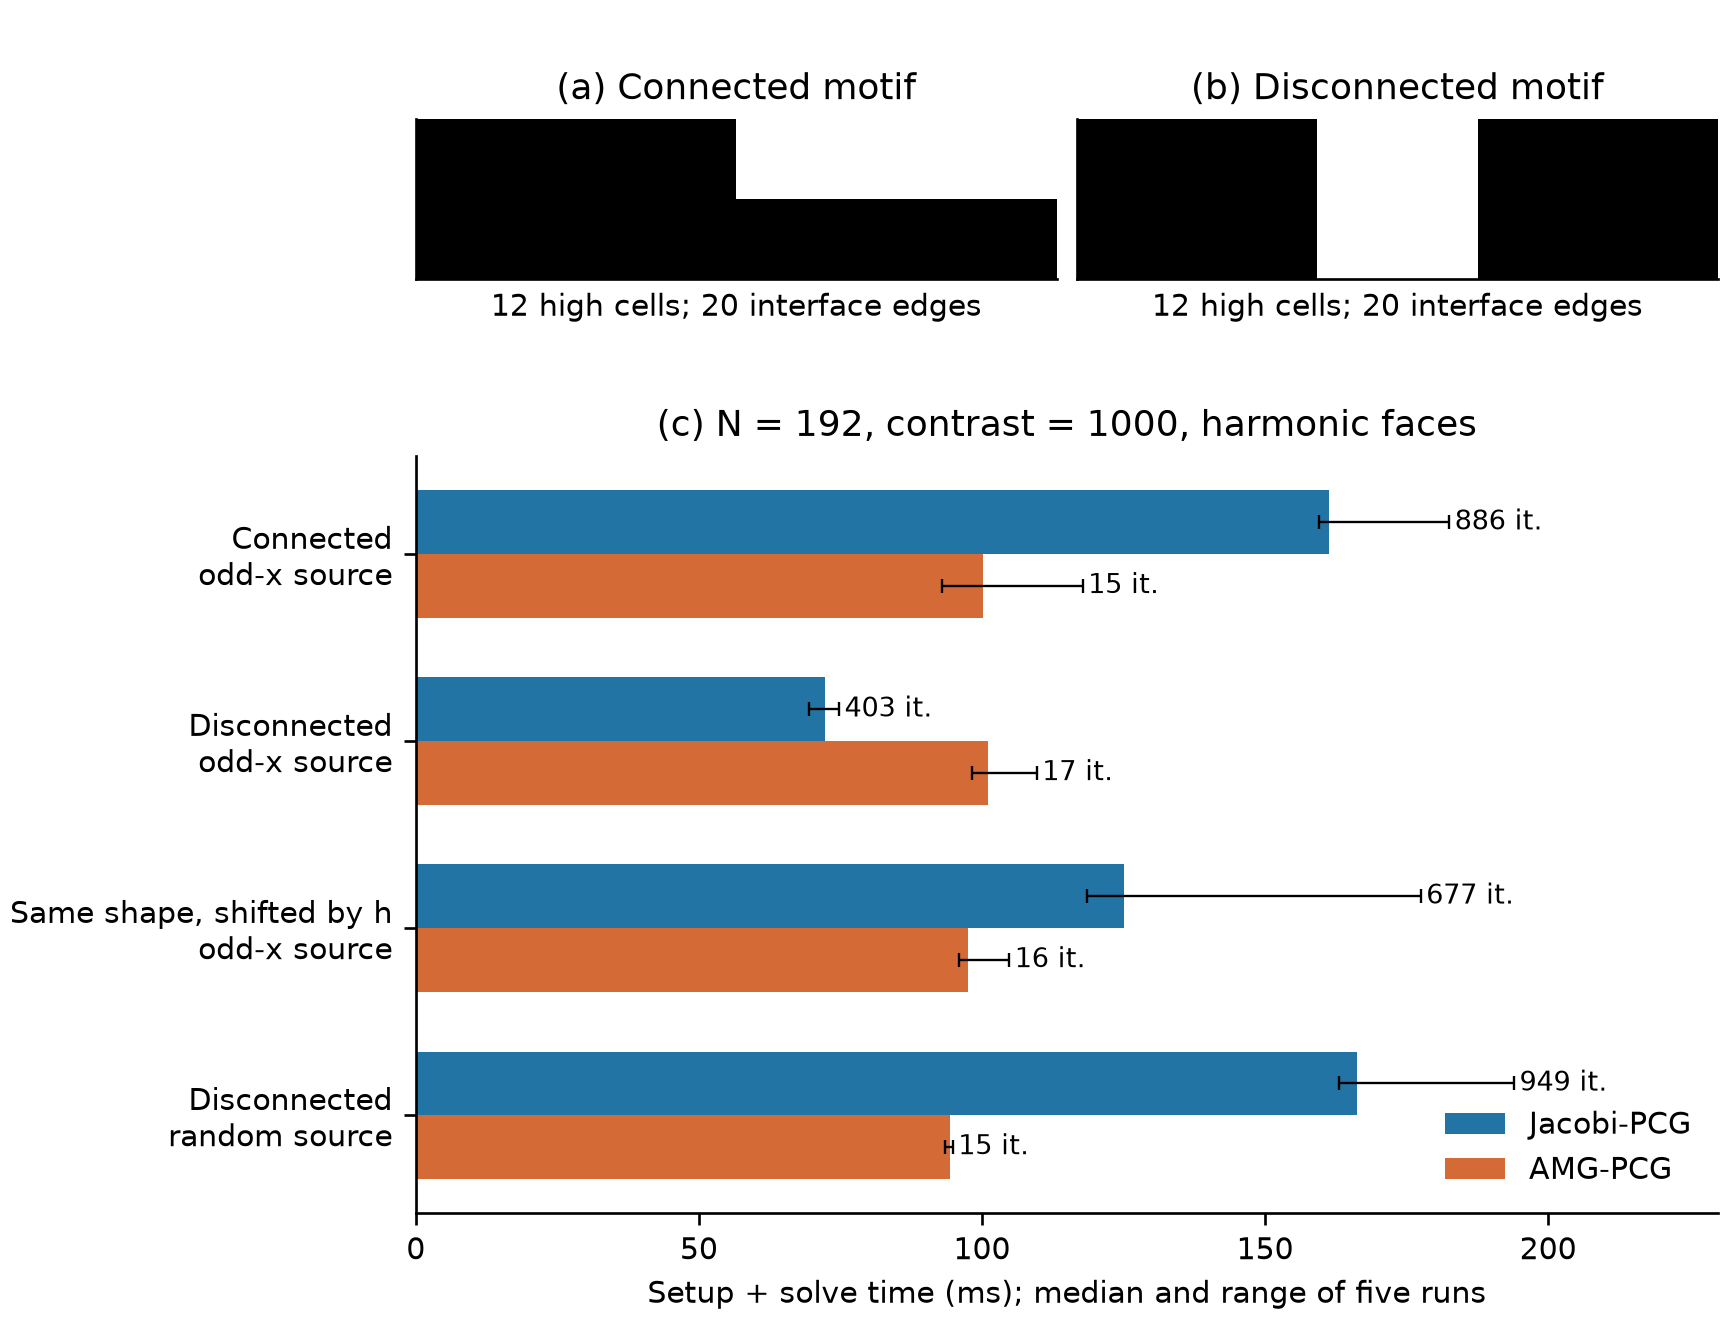
\includegraphics[width=\linewidth]{figures/counterfactual_audit.png}
\caption{Matched coefficient motifs and the forcing/translation audit. Bars show median setup-plus-solve times; whiskers span five runs. Iteration counts are annotated. The fields share scalar coefficient descriptors, while a rigid translation also preserves shape and connectivity.}
\label{fig:counterfactual}
\end{figure}

Controlled protocol. Following an exploratory 576-solve screen, confirmation uses c = 1000 and N = 96, 128, 192; centered, jointly transposed, and one-node x-shifted configurations; arithmetic and harmonic faces; and four unit-norm sources: constant, sin(2 pi x)sin(pi y), sin(pi x)sin(2 pi y), and a fixed-seed Gaussian vector. Jacobi-PCG and default SA-PCG each use five fresh setups per case, paired recorded setup seeds, shuffled method/source order, warm imports, and one BLAS thread. SA uses symmetric strength with theta = 0 and retains hierarchy diagnostics (keep=True). Count-only callbacks avoid the baseline residual-monitor overhead. CG uses rtol = 1e-9, zero initial guess, and at most 8000 iterations; an independent true relative residual must be at most 1e-8. Assembly and source construction are shared and excluded. The two timing protocols are not pooled.

A separate 3-by-6 motif family samples four connected and four disconnected patterns before observing their solver outcomes, retaining 12 occupied cells and 20 interface edges. It supplies 640 solves at N = 128, 192. This is a balanced constructed family, not a random sample of engineering materials. An additional 132-solve perturbation study varies translation direction and source admixtures with three repeats. The 1440 confirmation, 640 independent-family, and 132 perturbation solves all pass the true-residual check; the largest residual is below 3e-9. The pilot archive retains 84 failed acceptance checks, mainly at higher contrast or the CG iteration limit. No failed pilot timing is relabelled as a successful solve.

Mechanism. Let R reflect interior nodes in x and let D be the diagonal of A. If RA = AR, then R also commutes with D and the symmetrically scaled matrix S. For an odd source Rb = -b, every vector in the zero-start Krylov space generated by S and the scaled source g is odd. It is orthogonal to x-even eigenvectors in exact arithmetic. The centered two-island field satisfies this identity; its two slowest Jacobi-scaled modes are x-even. At N = 64 and c = 10000, computed squared source overlaps are below 1e-30 for both face averages. A transpose of both operator and source preserves Jacobi iteration counts, whereas translating the field in x breaks the reflection identity. This is a standard invariant-subspace explanation, not new convergence theory.

\begin{equation}
 S=D^{-1/2}AD^{-1/2},\qquad g=D^{-1/2}b,\qquad Rb=-b.
\end{equation}



Figure~\ref{fig:counterfactual} shows a concrete decision consequence at N = 192 with harmonic faces and c = 1000. For the odd-x source, the centered two-island field takes 403 Jacobi iterations and 72.2 ms, versus 17 AMG-PCG iterations and 101.0 ms. A one-node x translation increases Jacobi to 677 iterations and 125.1 ms, while AMG-PCG takes 16 iterations and 97.5 ms. Each winner is unchanged across the five repeats. With the same centered operator but a random source, Jacobi takes 949 iterations and 166.2 ms, and AMG-PCG takes 15 iterations and 94.3 ms. These are measured medians on this workstation, not universal crossover thresholds.

The full confirmation has a consistent per-repeat winner in 124 of 144 cells; the independent motif family has 55 of 64. Only two of the 48 centered-versus-x-shifted pairs reverse their winner consistently in all five repeats, so the reversal is a counterexample rather than a population-frequency claim. For the odd-x example within the Jacobi/SA portfolio, any deterministic rule restricted to the preserved coefficient invariants must choose the same method for both positions. Let T(j,s) be the median setup-plus-solve time for position j and candidate s in portfolio P. The least excess cost of a fixed choice across the equally weighted pair is E(P), defined below. For the two-method example, 1 + E(P) = 1.142. This empirical floor is not a statistical lower confidence bound, a bound for other solver portfolios, or a proposed selector. The raw tables include all pairs, unstable cells, and both methods.
\begin{equation}
 E(P)=\min_{s\in P}\left[\frac{1}{2}\sum_{j=0}^{1}
 \frac{T(j,s)}{\min_{t\in P}T(j,t)}\right]-1.
 \label{eq:empirical-floor}
\end{equation}


Source perturbations test the interpretation without changing A: at N = 192, adding a constant component of amplitude 1e-8 to the unit odd source raises Jacobi from 403 to 569 iterations under the same stopping tolerance. A y translation preserves x reflection but can change the remaining spectrum and other symmetry sectors; parity alone is therefore not a complete runtime predictor. Offline spectra use symmetric Jacobi scaling and the nonsymmetric operator BA for the AMG inverse preconditioner B. Small-grid dense symmetrisation checks validate the numerical spectral procedure. Neither eigenvalue computations nor the reflection audit is included in a claimed low-cost selection policy.

Candidate-solver sensitivity. A separate 240-solve screen adds SA with symmetric-strength theta = 0.25 and classical Ruge-Stueben AMG with classical strength theta = 0.25. A subsequent 504-solve confirmation compares Jacobi, SA with theta = 0, and classical AMG at N = 128, 160, 192, using the two-island motif and the previously tested symmetric 3-by-6 anchor, whose three rows are each 110011. Each of seven repeats interleaves both field positions, both sources, both motifs, and all three methods at a fixed N. All 744 solves pass the same residual acceptance check; their timings are not pooled with earlier stages. The confirmation has 17 of 24 cells with the same winner in every repeat, and three of 12 translated pairs reverse their winner in all seven repeats. Table~\ref{tab:portfolio-audit} reports all 12 pairs, including unstable cells and zero floors. For the original motif at N = 128 with odd-x forcing, centered Jacobi and classical AMG take 24.3 and 36.8 ms; after translation they take 42.3 and 34.2 ms. Jacobi iterations rise from 266 to 450, while classical AMG takes 11 in both positions. The three-method empirical excess-cost floor for this pair is 11.91%. At N = 192, classical AMG has the lowest median time at both positions, giving zero median-based floor for that pair, although the centered winner is not identical in all repeats. Thus translation sensitivity survives a stronger baseline, but its measured decision boundary and cost consequence depend on the candidate solver set.

\begin{table}[t]
\centering
\caption{All 12 translated pairs in the interleaved confirmation. Winners use median total time: J = Jacobi-PCG, RS = classical AMG-PCG; SA was also a candidate. Stable means both positions retain their respective winner in all seven repeats. E(P) uses measured medians even for unstable pairs; it is not a confidence bound.}
\label{tab:portfolio-audit}
\begin{tabular}{rlllllr}
\toprule
$N$ & Motif & Source & Centered & Shifted & Stable & $E(P)$ (\%) \\
\midrule
128 & 3x6 & Odd-x & J & RS & Yes & 12.42 \\
128 & 3x6 & Random & RS & RS & Yes & 0.00 \\
128 & 2x8 & Odd-x & J & RS & Yes & 11.91 \\
128 & 2x8 & Random & RS & RS & Yes & 0.00 \\
160 & 3x6 & Odd-x & J & RS & Yes & 9.69 \\
160 & 3x6 & Random & RS & RS & No & 0.00 \\
160 & 2x8 & Odd-x & J & RS & No & 4.86 \\
160 & 2x8 & Random & RS & RS & Yes & 0.00 \\
192 & 3x6 & Odd-x & RS & RS & No & 0.00 \\
192 & 3x6 & Random & RS & RS & Yes & 0.00 \\
192 & 2x8 & Odd-x & RS & RS & No & 0.00 \\
192 & 2x8 & Random & RS & RS & Yes & 0.00 \\
\bottomrule
\end{tabular}
\end{table}


\subsection{CPU and CUDA Stencil Scaling}

At $N=2048$, NumPy required 0.1813 s per apply, while Numba serial required 0.005325 s and Numba parallel with four threads required 0.003725 s. Increasing thread count beyond four did not improve the largest case in this run; the measurements alone do not distinguish memory-system limits from scheduling overhead.

The CUDA Jacobi benchmark measures the resident-data update cost. At $N=512$, GPU and CPU kernel times were essentially equal. At $N=1024$, CUDA reached $1.52\times$ speedup. At $N=2048$ and $N=4096$, the speedups increased to $3.23\times$ and $3.51\times$, respectively. The measurements describe this kernel and workstation. They do not imply the same speedup for an end-to-end sparse solver.

\begin{table}[t]
\centering
\caption{Representative stencil-throughput measurements. CPU entries use the variable-coefficient operator at $N=2048$; CUDA entries use a repeated Jacobi kernel-only benchmark.}
\label{tab:performance}
\resizebox{\columnwidth}{!}{%
\begin{tabular}{llrrr}
\toprule
Experiment & Method & $N$ & Time & Throughput / speedup \\
\midrule
CPU stencil & NumPy & 2048 & 0.1813 s/apply & 2.03 GB/s \\
CPU stencil & Numba serial & 2048 & 0.005325 s/apply & 69.18 GB/s \\
CPU stencil & Numba parallel, 4 threads & 2048 & 0.003725 s/apply & 98.90 GB/s \\
GPU crossover & CUDA kernel & 2048 & $7.97\times10^{-4}$ s/step & $3.23\times$ vs CPU \\
GPU crossover & CUDA kernel & 4096 & $3.15\times10^{-3}$ s/step & $3.51\times$ vs CPU \\
\bottomrule
\end{tabular}
}
\end{table}


\begin{figure}[t]
\centering
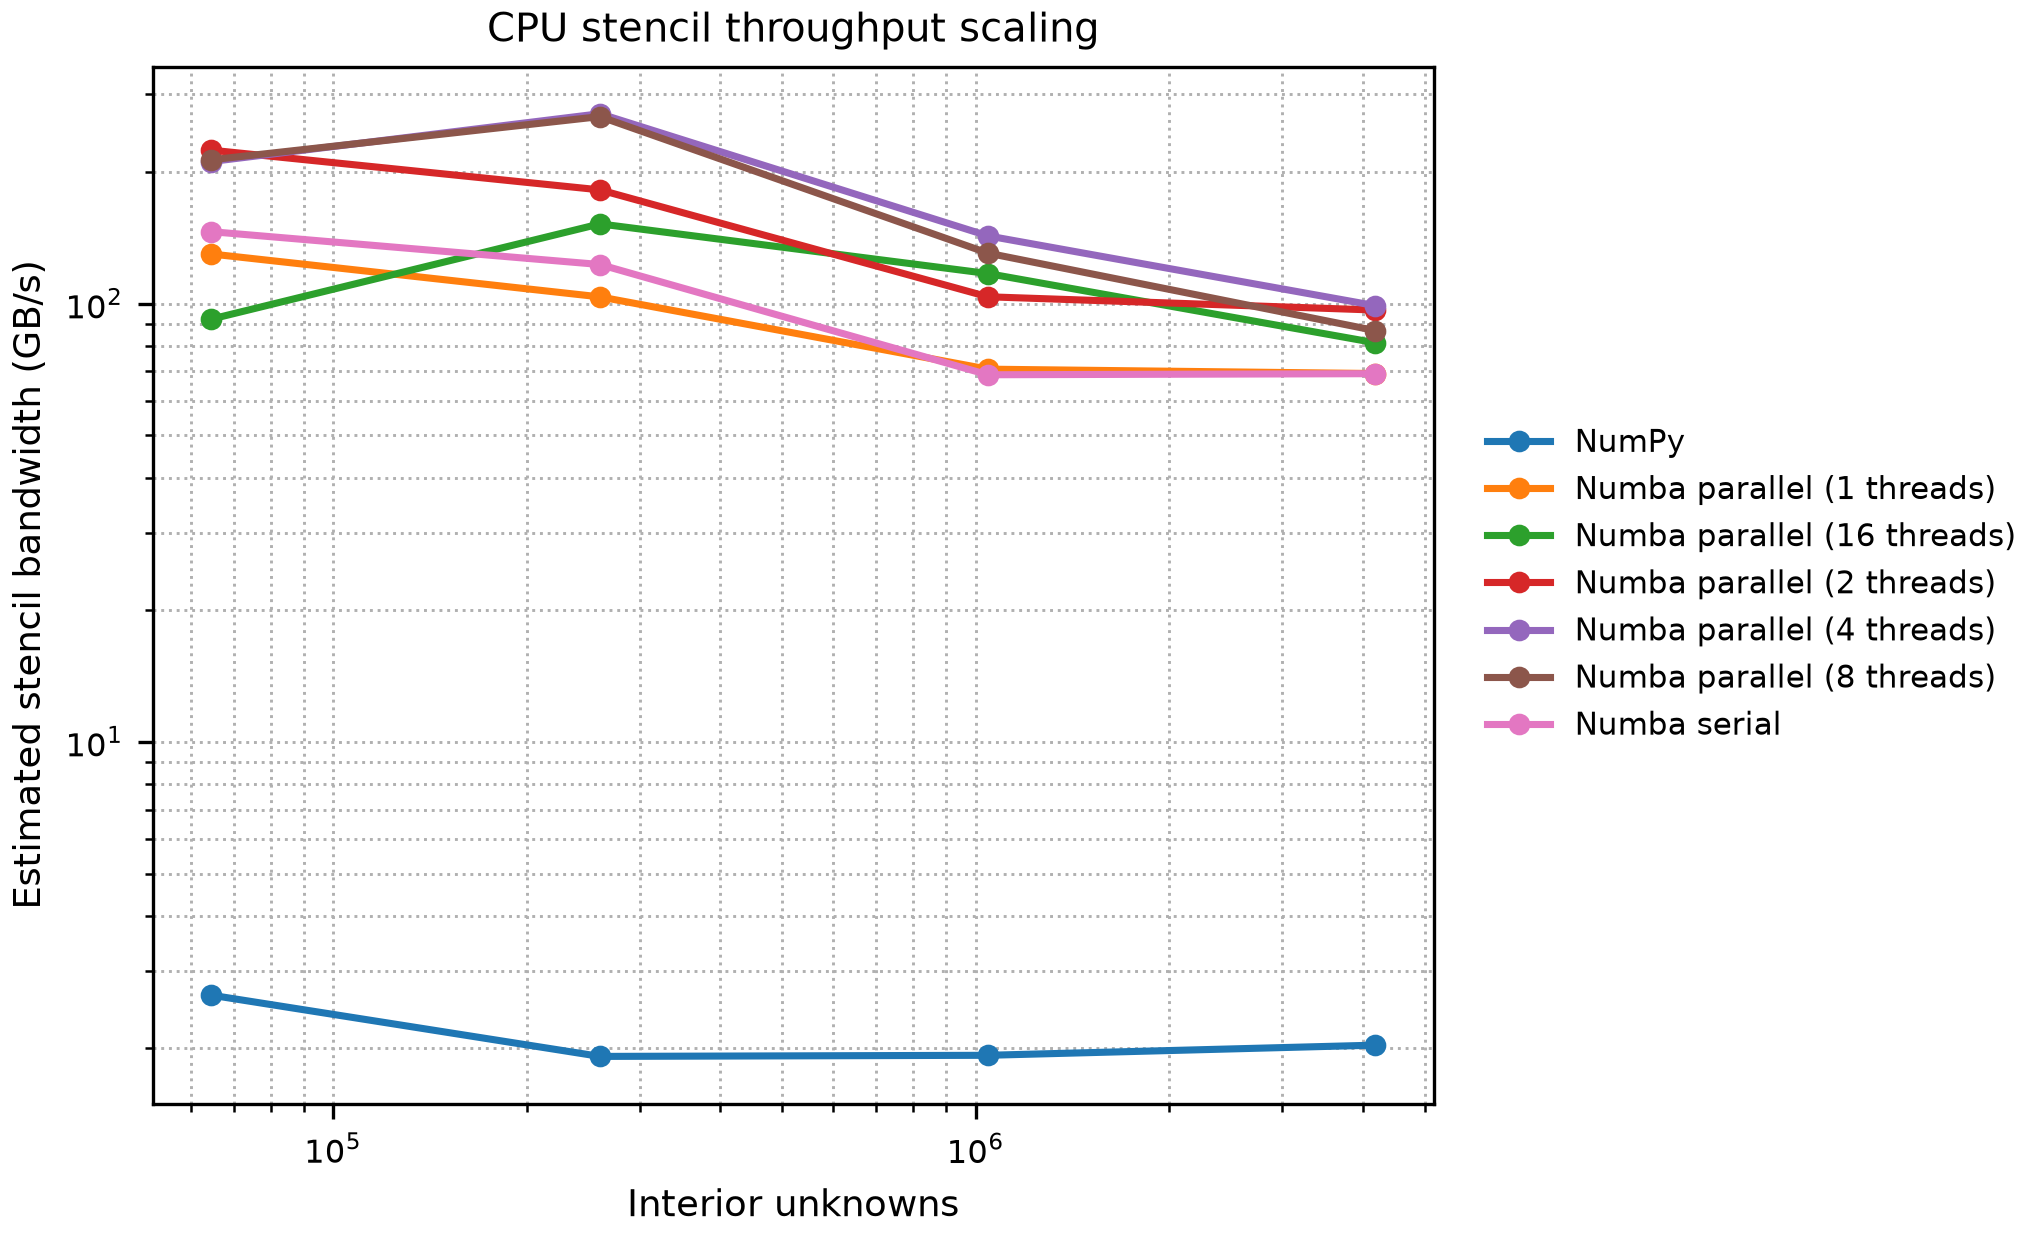
\includegraphics[width=0.84\linewidth]{figures/cpu_scaling.png}
\caption{Estimated CPU stencil bandwidth for the variable-coefficient stencil apply.}
\label{fig:cpu_scaling}
\end{figure}

\begin{figure}[t]
\centering
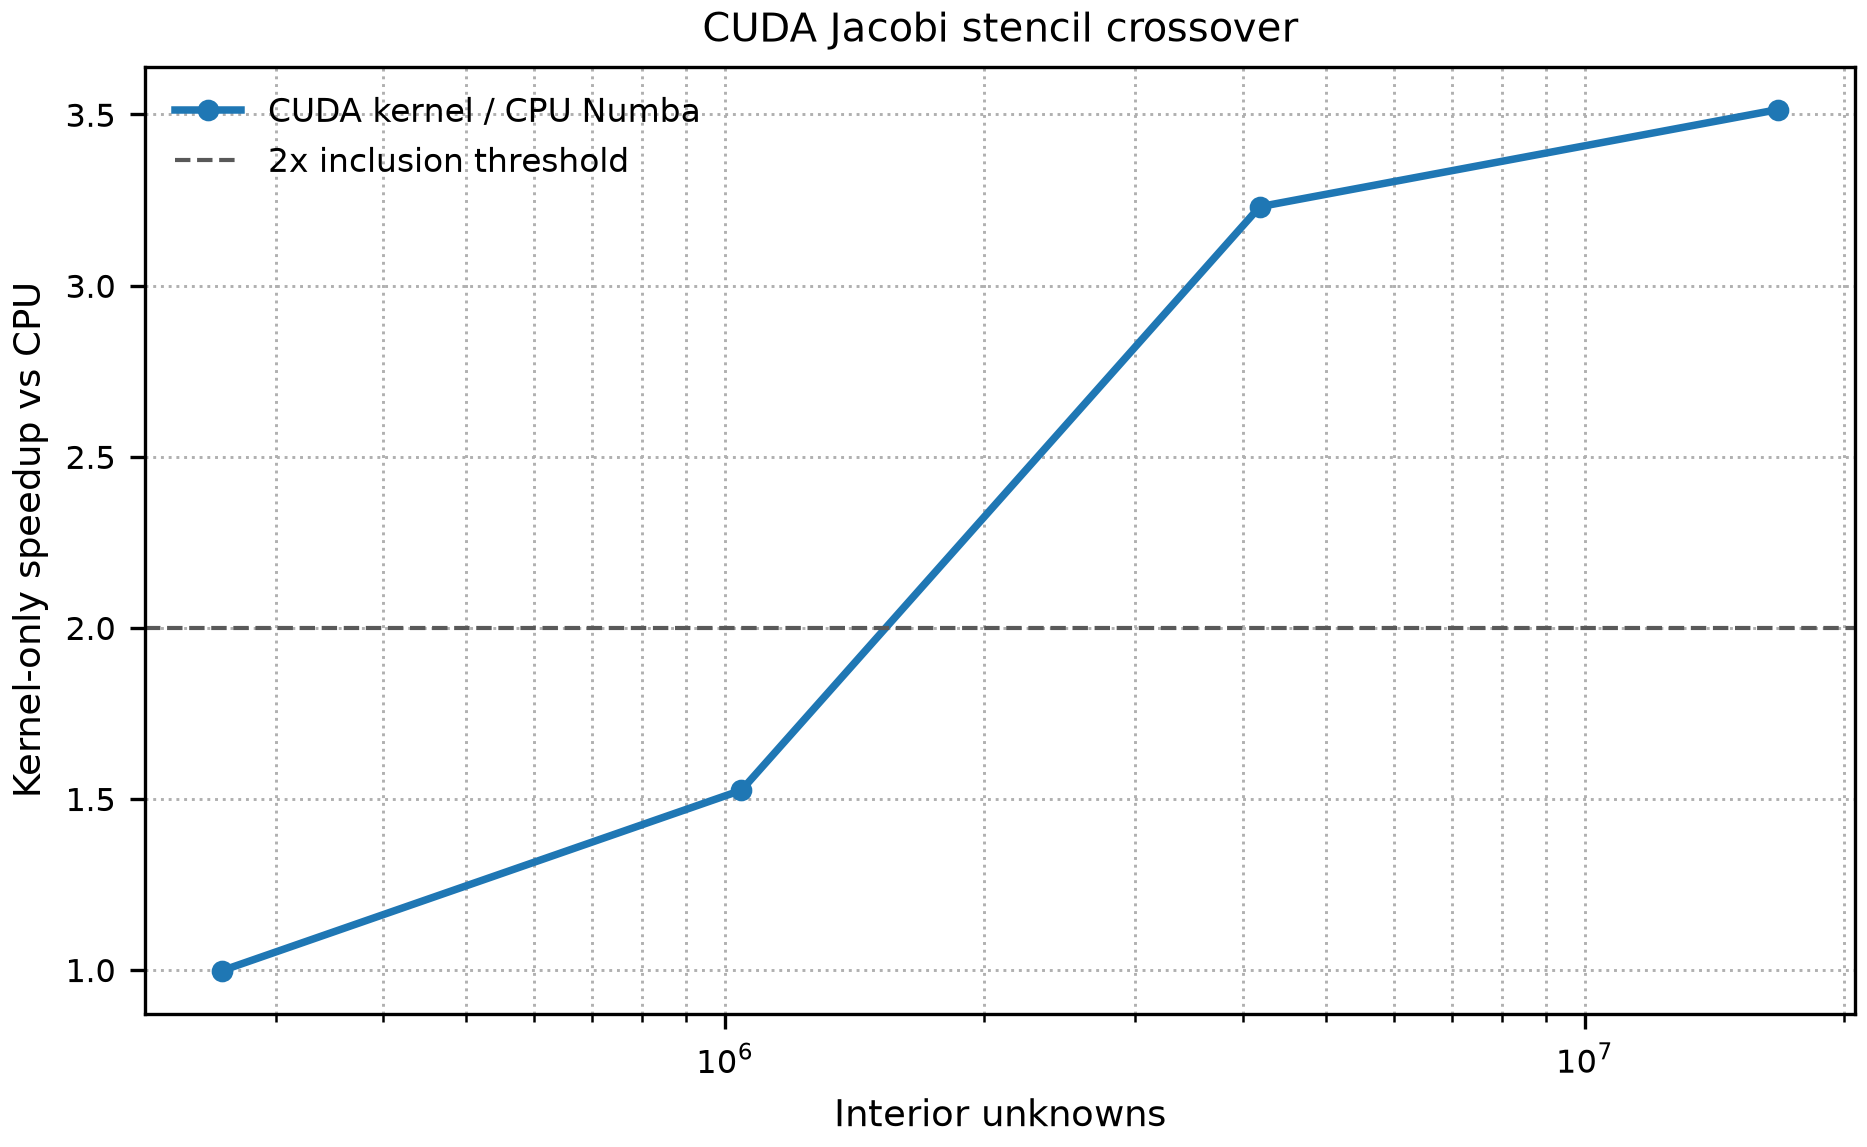
\includegraphics[width=0.84\linewidth]{figures/gpu_crossover.png}
\caption{CUDA kernel-only speedup for repeated Jacobi updates relative to a four-thread Numba CPU baseline.}
\label{fig:gpu_crossover}
\end{figure}

The measured timings are approximately equal at N = 512, and CUDA is faster at N = 1024. The supplementary artefact retains the exploratory four-point linear fit. Its negative CPU-time prediction at the measured N = 512 point invalidates its use as a crossover-location estimate; no fitted hardware-selection threshold is claimed.

\section{Discussion}

The matched-field audit qualifies the baseline resolution-dependent decision map. The original monitored runs show the expected setup-versus-iteration trade-off, but their uniform winner at each resolution does not establish descriptor sufficiency. In the controlled extension, a rigid translation or a source perturbation changes the effective Krylov workload while retaining the listed coefficient invariants. The practical recommendation is to test forcing, alignment, and candidate-solver sensitivity before interpreting a coefficient-stratified timing map as a reusable decision rule. The classical-AMG check shows why a cost floor established for two methods must be recomputed when the portfolio changes. Symmetric sources can be physically appropriate; their fast solves should be reported as workload-specific evidence, not treated as an error or extrapolated to arbitrary forcing.

For physical composite-conduction use, the face law must be chosen from the interface geometry and resistance model before comparing solvers. The arithmetic benchmark is not evidence of accurate cross-interface flux at high contrast. For performance use, the callback calibration shows that an iteration monitor can disproportionately penalise inexpensive iterations; solver rankings and their uncertainty must therefore be reported with the callback, setup and execution protocol.

The coefficient descriptors are empirical summaries, not conditioning theory. Their uncertainty intervals overlap, and small fixed-grid strata do not establish a reliable ordering of predictive importance. Pooled correlations also reflect resolution; N = 256 uses an N = 128 condition estimate. Case-resampling intervals describe sensitivity to this constructed dataset, not population confidence or performance on unseen geometries.

The stencil measurements demonstrate implementation and size effects. Nonmonotone CPU scaling is consistent with bandwidth or scheduling limits, but no hardware counters separate these causes. CUDA timings include launch and final synchronisation with data resident on the device. They exclude transfer costs and full sparse solves; the four-point fit cannot validate a crossover threshold.

The scope is two-dimensional structured grids, synthetic coefficients and one workstation. Harmonic averaging does not resolve curved interfaces cutting grid cells. Industrial geometries, unstructured finite elements and transient multiphysics remain outside the evidence. The contribution is a reproducible audit of numerical correctness and conditional solver costs, not production solver robustness.

\section{Reproducibility Artefact}

The previously published baseline and controlled extension are archived at \url{https://doi.org/10.5281/zenodo.22668106}, with the earlier baseline at \url{https://doi.org/10.5281/zenodo.22303525}. The present revision additionally supplies the callback calibration in \path{results/raw/protocol_sensitivity}, its prospective protocol in \path{experiments/protocol_sensitivity.md}, and complete generated summaries in \path{results/analysis/protocol_sensitivity} through the accompanying supplementary package. The complete revised artefact, including these calibration files, is archived at \url{https://doi.org/10.5281/zenodo.22874266} (version v5). Raw histories are retained unchanged. Run \path{experiments/analyze_protocol_sensitivity.py} to regenerate the two new tables from the recorded CSV files. Recorded configurations and source hashes document the calibration. The reproduction instructions distinguish historical monitored runs from controlled count-only runs and preserve pilot failures. Tests check flux-energy identities, matched descriptors, reflection invariance and transpose equivalence. CPU-only tests explicitly skip unavailable CUDA tests; CUDA-required mode treats missing GPU support as an error. Timing reruns may differ with machine state.

\section{Conclusion}

In the controlled heat-conduction tests, preserving scalar coefficient descriptors, shape and connectivity does not guarantee the same fastest solver: source and alignment changes can alter the measured setup-inclusive choice. The classical-AMG comparison shows that the reversal also depends on the candidate solver set. These findings support checking forcing, alignment and candidate solvers before reusing a coefficient-based decision map, alongside operator verification, complete setup timing and retention of failed solves. The CPU/CUDA experiments provide separate stencil measurements, with GPU results limited to resident data on the tested workstation. The study introduces no new numerical algorithm or universal selection rule.

\section*{Acknowledgements}

The author used OpenAI GPT-5 for editorial assistance and DeepSeek V4 Pro through Claude Code for language polishing. OpenAI GPT-6 Astra assisted with experimental design, code implementation, numerical analysis and manuscript preparation. The author independently reviewed the controlled experiments, including their derivations, timing boundaries and failure cases, and takes responsibility for the code, results, references and final manuscript.

\bibliographystyle{unsrt}
\bibliography{references}

\end{document}
